\documentclass[tikz,border=8pt]{standalone}
\usepackage{amsmath,amssymb}
\usetikzlibrary{arrows.meta,automata,positioning,quotes}
\begin{document}
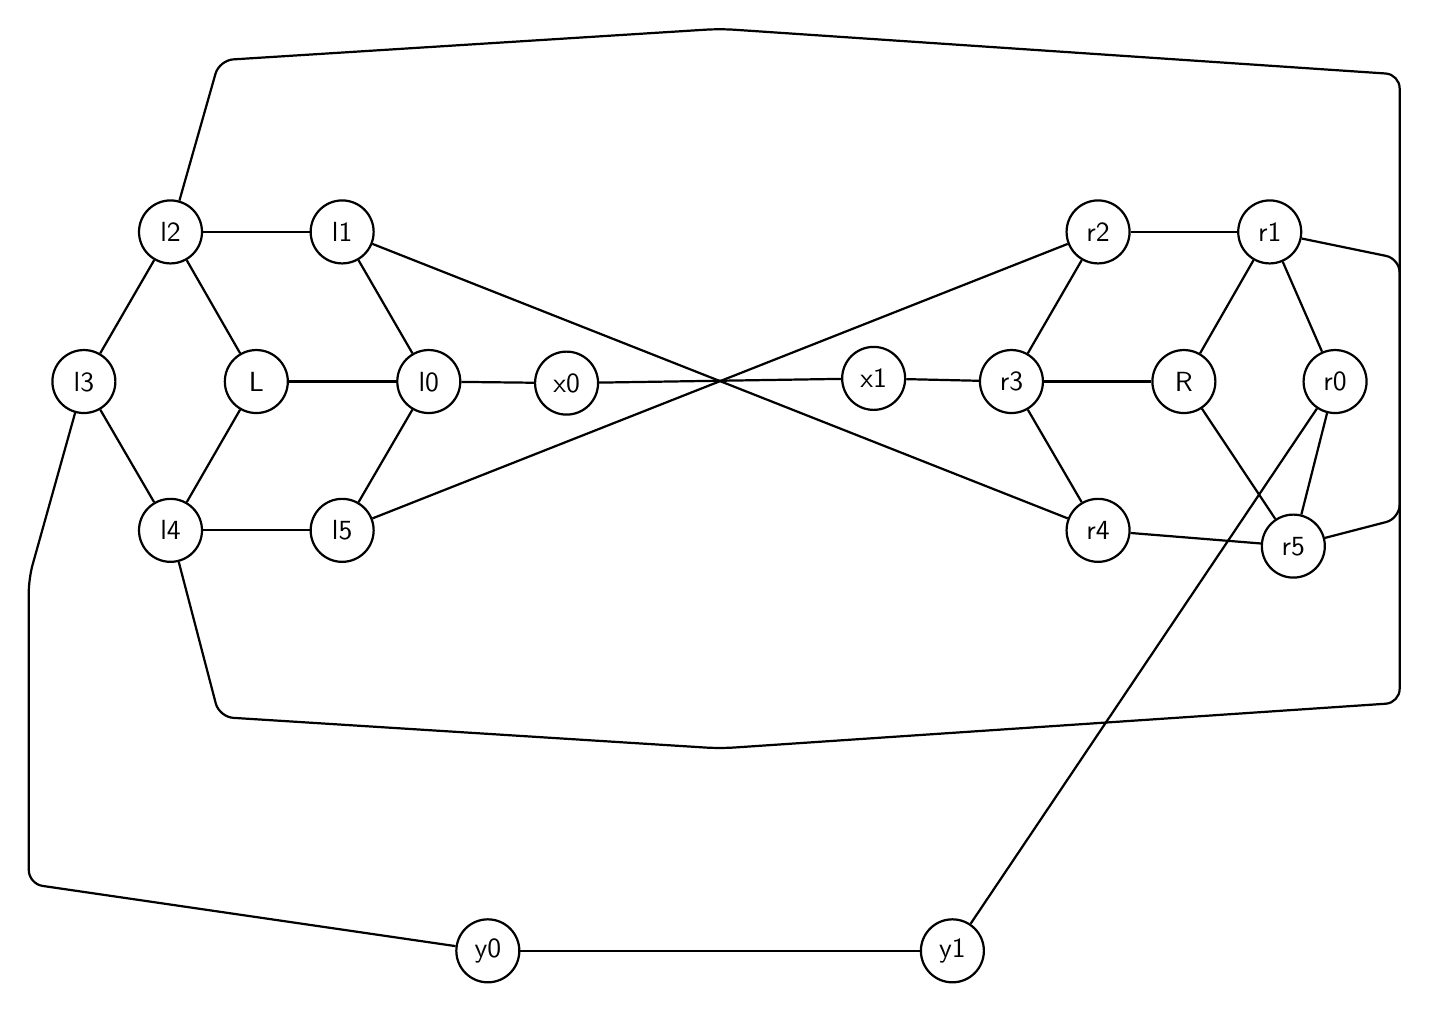
\begin{tikzpicture}[x=1cm,y=1cm]
\tikzset{
  graphnode/.style={circle,draw,thick,minimum size=8mm,inner sep=1pt,font=\sffamily},
  directed/.style={-{Stealth[length=2.4mm]},thick},
  undirected/.style={thick}
}
\node[graphnode] (n_L) at (-6.11,0.95) {L};
\node[graphnode] (n_l0) at (-3.92,0.95) {l0};
\node[graphnode] (n_l1) at (-5.02,2.85) {l1};
\node[graphnode] (n_l2) at (-7.20,2.85) {l2};
\node[graphnode] (n_l3) at (-8.30,0.95) {l3};
\node[graphnode] (n_l4) at (-7.20,-0.94) {l4};
\node[graphnode] (n_l5) at (-5.02,-0.94) {l5};
\node[graphnode] (n_R) at (5.67,0.95) {R};
\node[graphnode] (n_r0) at (7.59,0.95) {r0};
\node[graphnode] (n_r1) at (6.76,2.85) {r1};
\node[graphnode] (n_r2) at (4.58,2.85) {r2};
\node[graphnode] (n_r3) at (3.48,0.95) {r3};
\node[graphnode] (n_r4) at (4.58,-0.94) {r4};
\node[graphnode] (n_r5) at (7.06,-1.14) {r5};
\node[graphnode] (n_x0) at (-2.17,0.93) {x0};
\node[graphnode] (n_x1) at (1.73,0.99) {x1};
\node[graphnode] (n_y0) at (-3.17,-6.28) {y0};
\node[graphnode] (n_y1) at (2.73,-6.28) {y1};
\draw[undirected] (n_l0) -- (n_l1);
\draw[undirected] (n_l1) -- (n_l2);
\draw[undirected] (n_l2) -- (n_l3);
\draw[undirected] (n_l3) -- (n_l4);
\draw[undirected] (n_l4) -- (n_l5);
\draw[undirected] (n_l5) -- (n_l0);
\draw[undirected] (n_L) -- (n_l0);
\draw[undirected] (n_L) -- (n_l2);
\draw[undirected] (n_L) -- (n_l4);
\draw[undirected] (n_r0) -- (n_r1);
\draw[undirected] (n_r1) -- (n_r2);
\draw[undirected] (n_r2) -- (n_r3);
\draw[undirected] (n_r3) -- (n_r4);
\draw[undirected] (n_r4) -- (n_r5);
\draw[undirected] (n_r5) -- (n_r0);
\draw[undirected] (n_R) -- (n_r1);
\draw[undirected] (n_R) -- (n_r3);
\draw[undirected] (n_R) -- (n_r5);
\draw[undirected] (n_l0) -- (n_x0);
\draw[undirected] (n_x0) -- (n_x1);
\draw[undirected] (n_x1) -- (n_r3);
\draw[undirected,rounded corners=5pt] (n_l3) -- (-9.00,-1.55) -- (-9.00,-5.43) -- (n_y0);
\draw[undirected] (n_y0) -- (n_y1);
\draw[undirected] (n_y1) -- (n_r0);
\draw[undirected] (n_l1) -- (n_r4);
\draw[undirected,rounded corners=5pt] (n_l2) -- (-6.58,5.03) -- (-0.22,5.43) -- (8.41,4.85) -- (8.41,-0.79) -- (n_r5);
\draw[undirected,rounded corners=5pt] (n_l4) -- (-6.58,-3.31) -- (-0.22,-3.71) -- (8.41,-3.13) -- (8.41,2.51) -- (n_r1);
\draw[undirected] (n_l5) -- (n_r2);
\end{tikzpicture}
\end{document}
